\subsection{Disappearance of ``Type B'' Parameter Regions}
\label{sec:add.change.disb}

For \Cref{fig:add.change.regions.1,fig:add.change.regions.2}, the ``type B'' parameter region $Q^{20}_3$ is complete.
In \Cref{fig:add.change.regions.4}, it is gone completely, instead the two ``type A'' parameter regions $P^{20}_3$ and $P^{20}_4$ now overlap.

\begin{figure}
	\centering
	\subfloat[Regions]{
		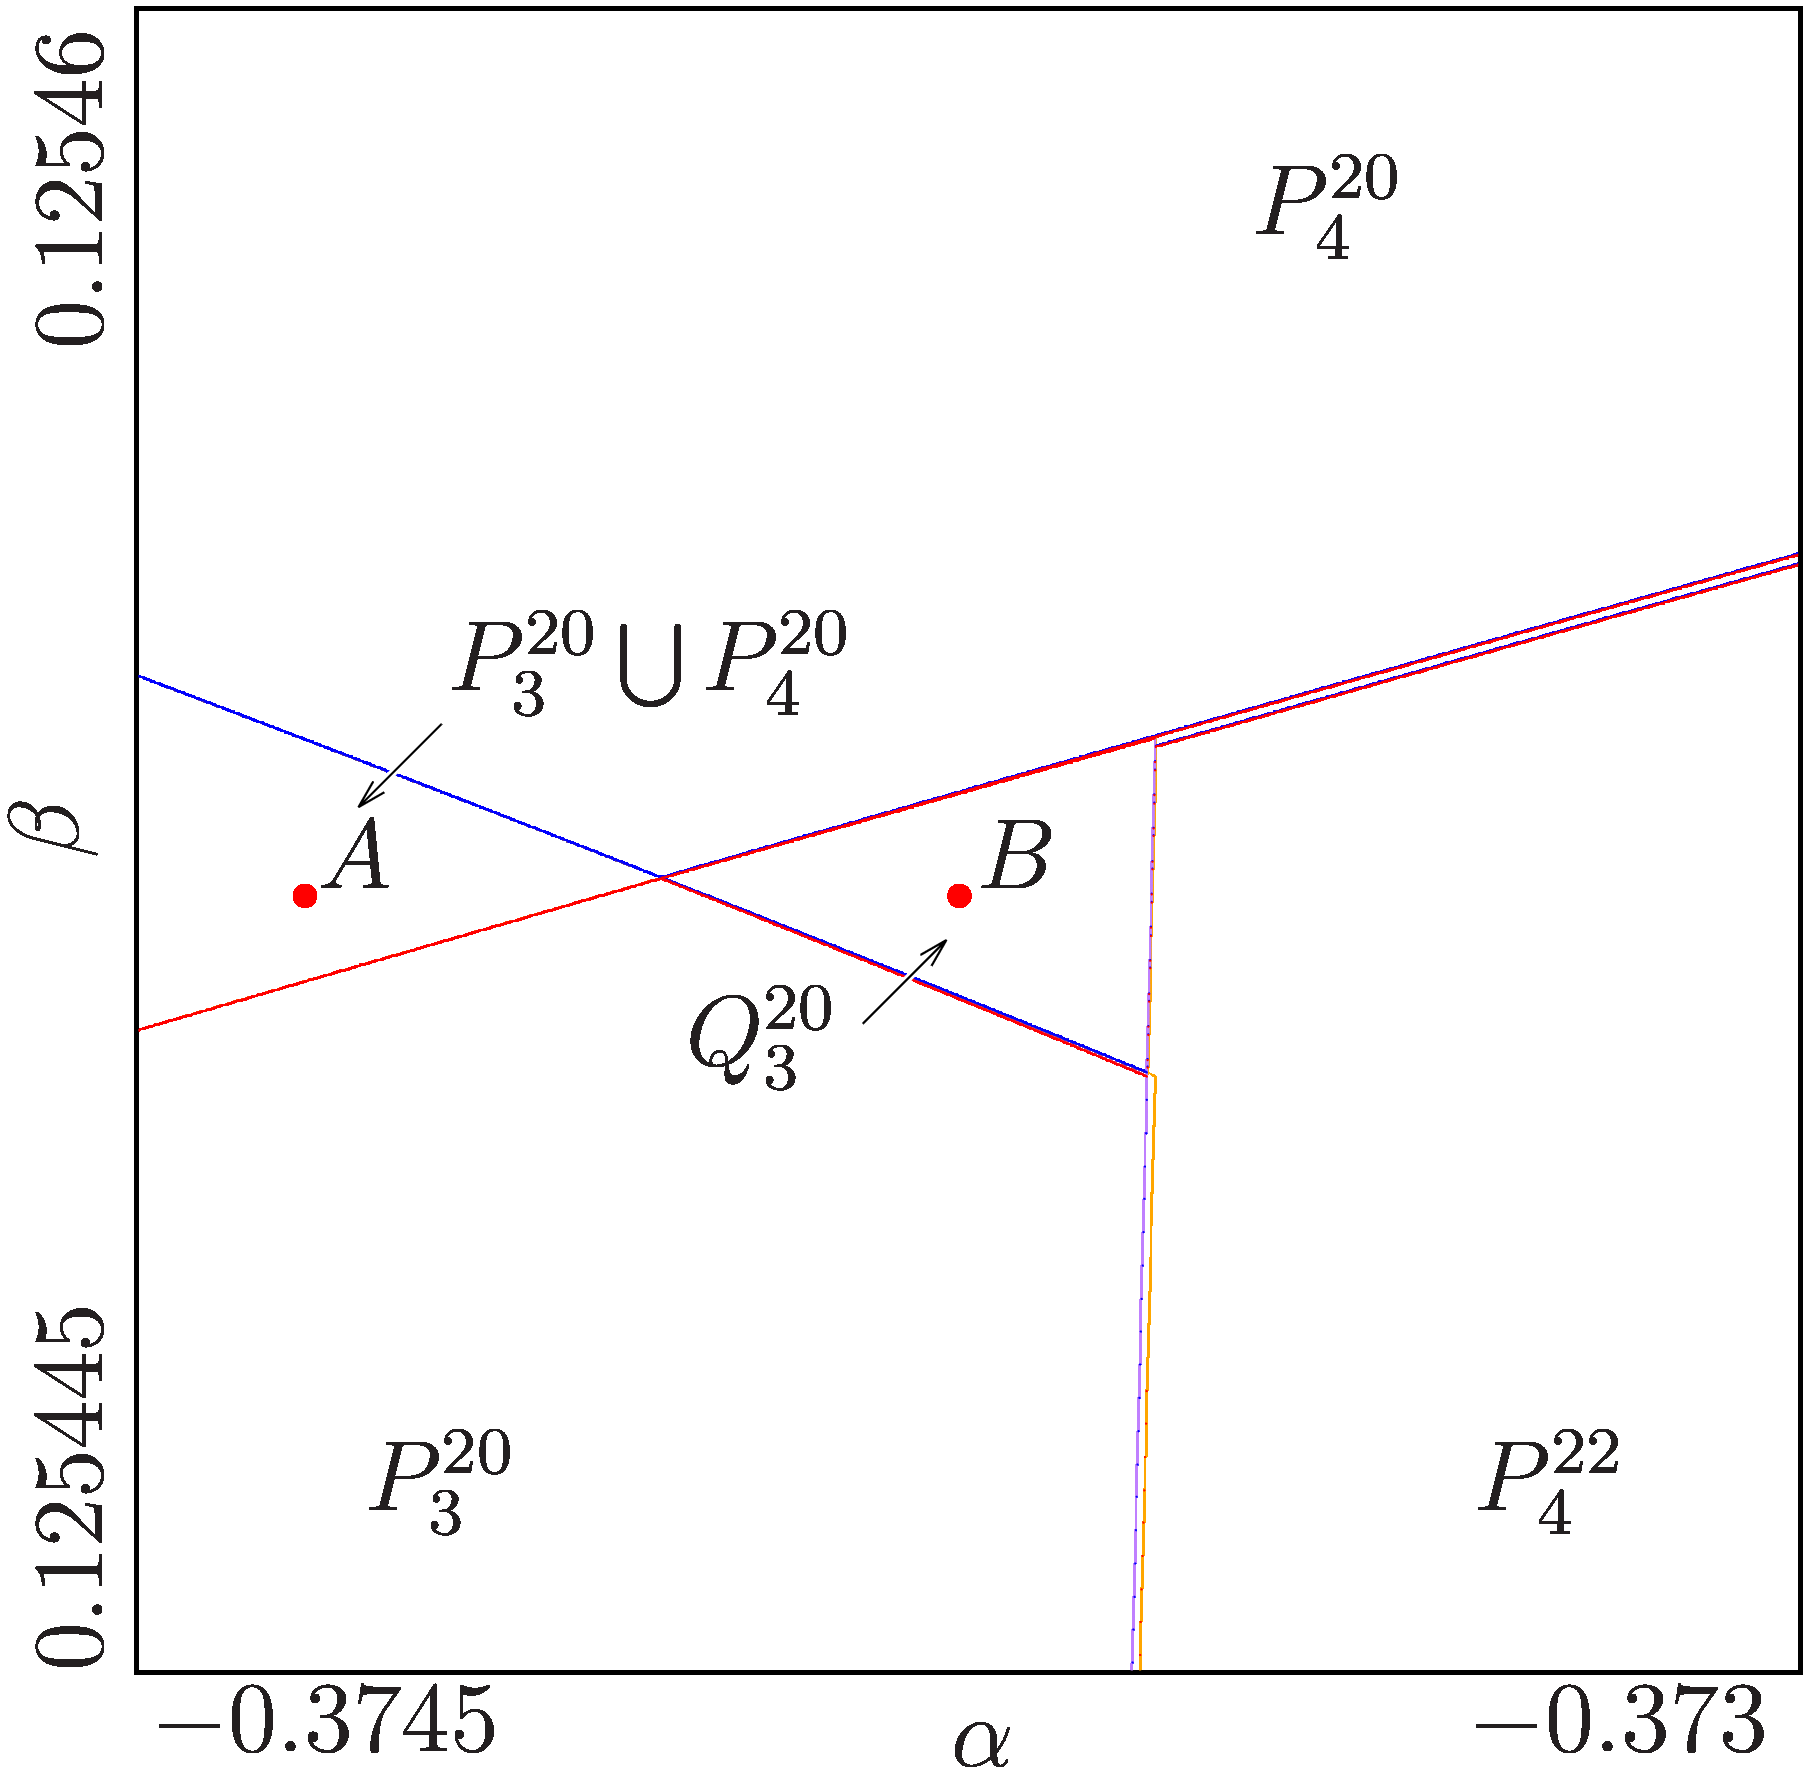
\includegraphics[width=.3 \textwidth]{../Figures/7/7.4a/result.png}
		\label{fig:add.change.disb.regions}
	}
	\subfloat[Cobweb at point $A$]{
		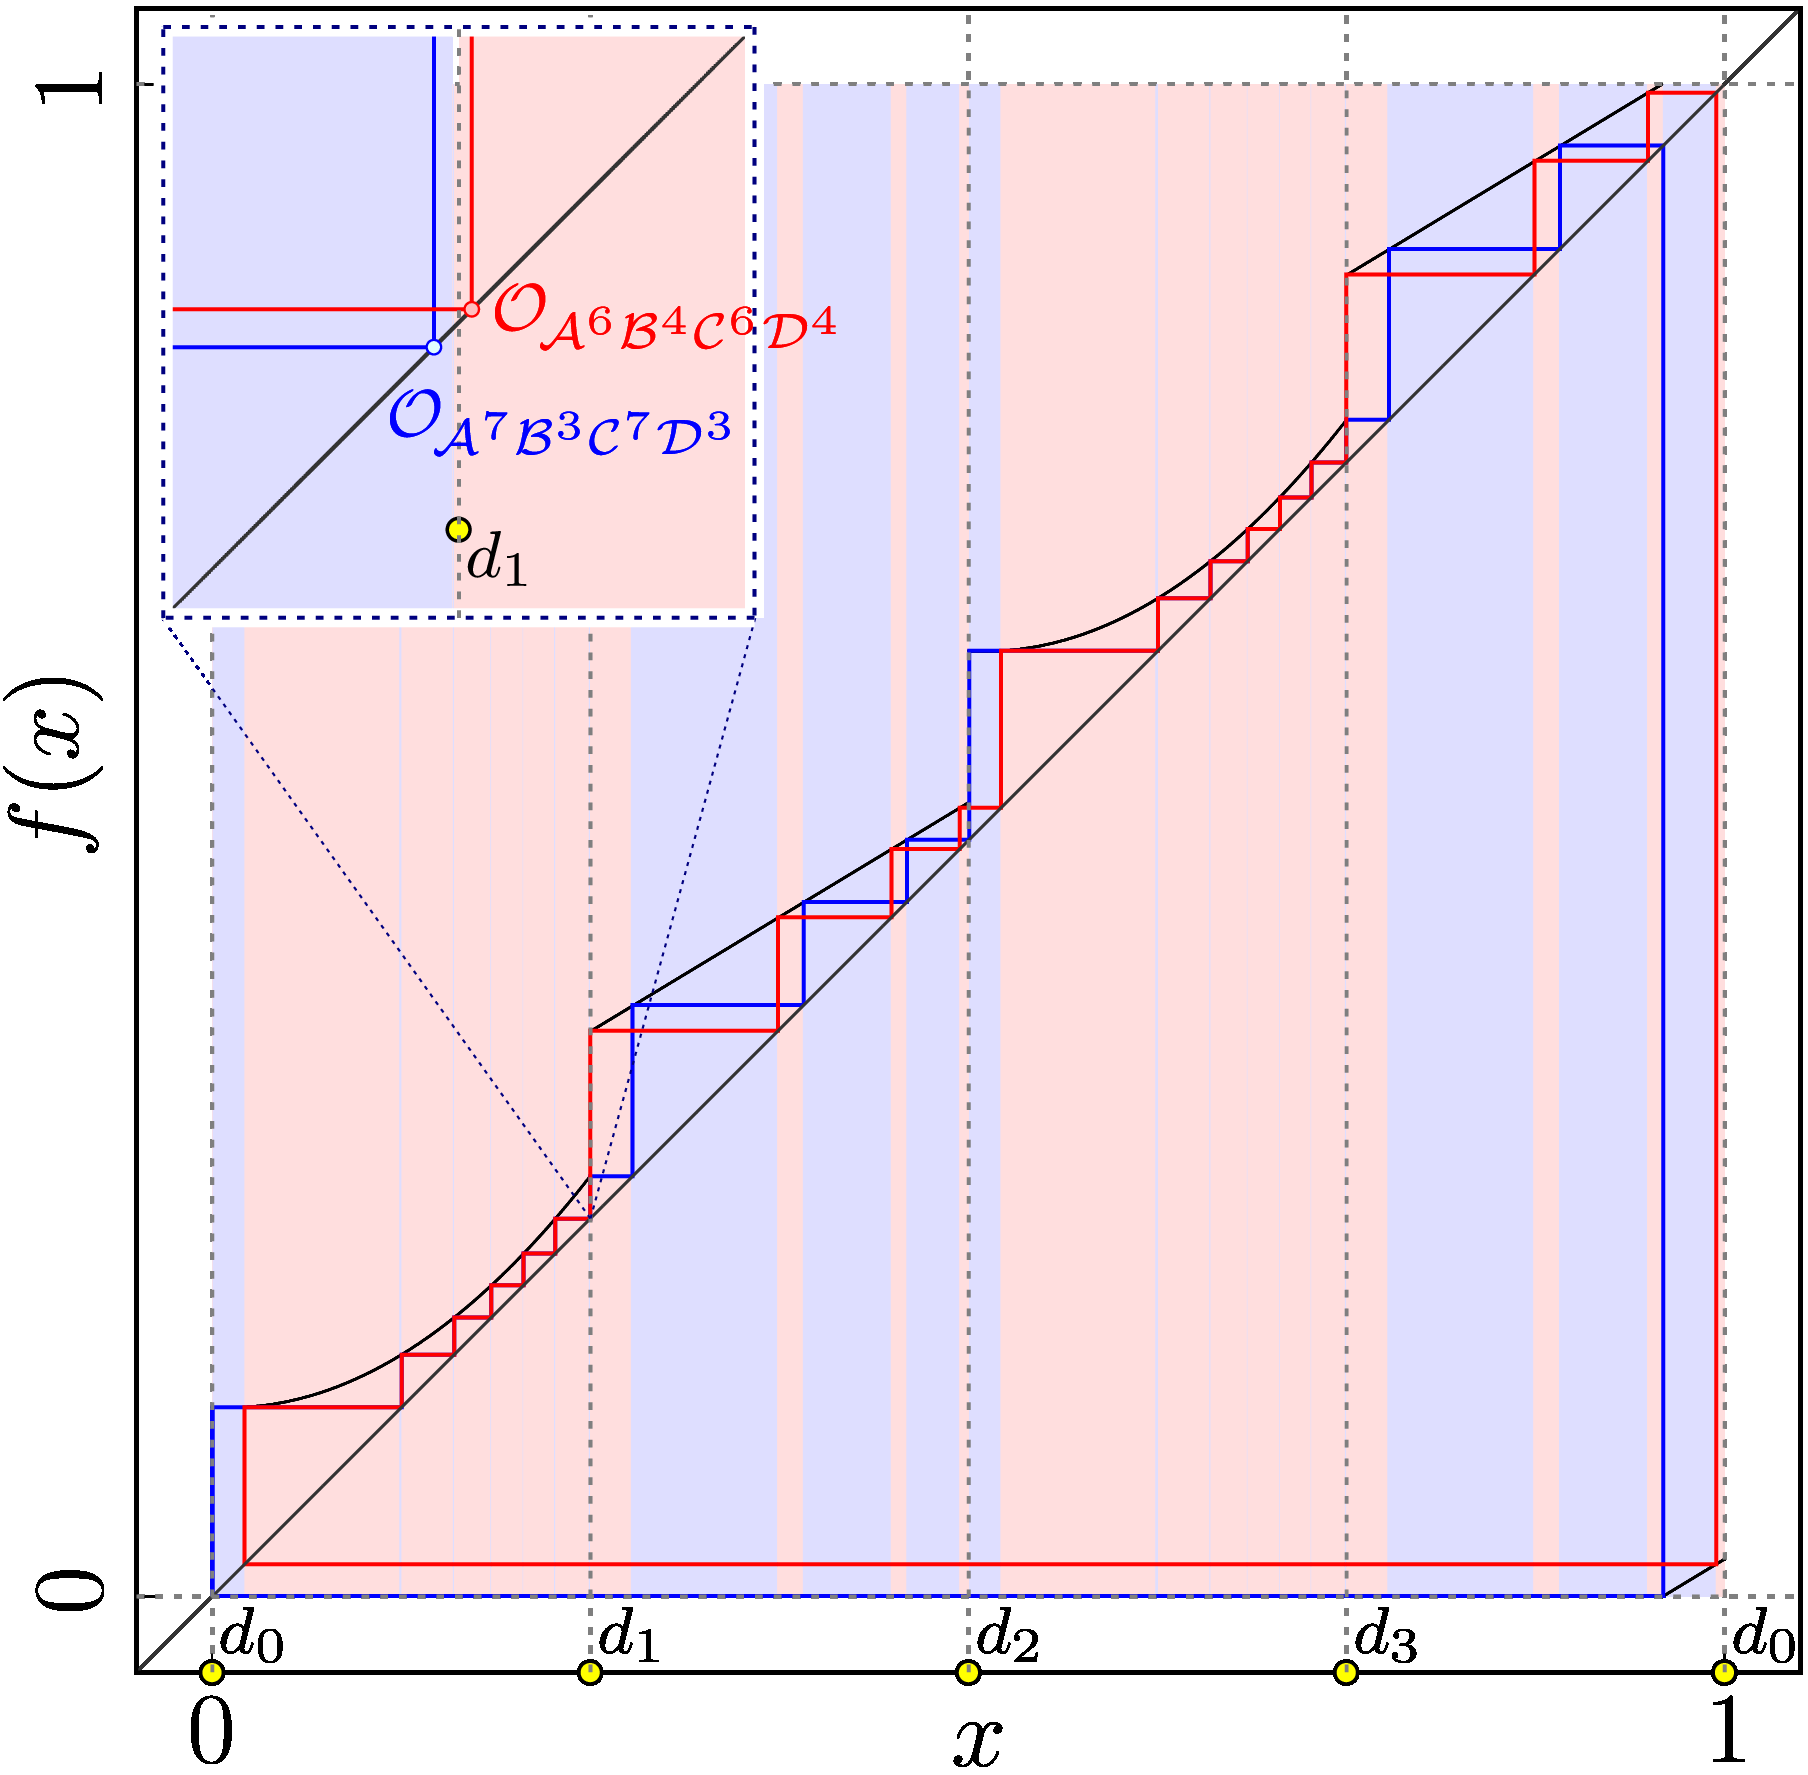
\includegraphics[width=.3 \textwidth]{../Figures/7/7.4b/result.png}
		\label{fig:add.change.disb.cob.A}
	}
	\subfloat[Cobweb at point $B$]{
		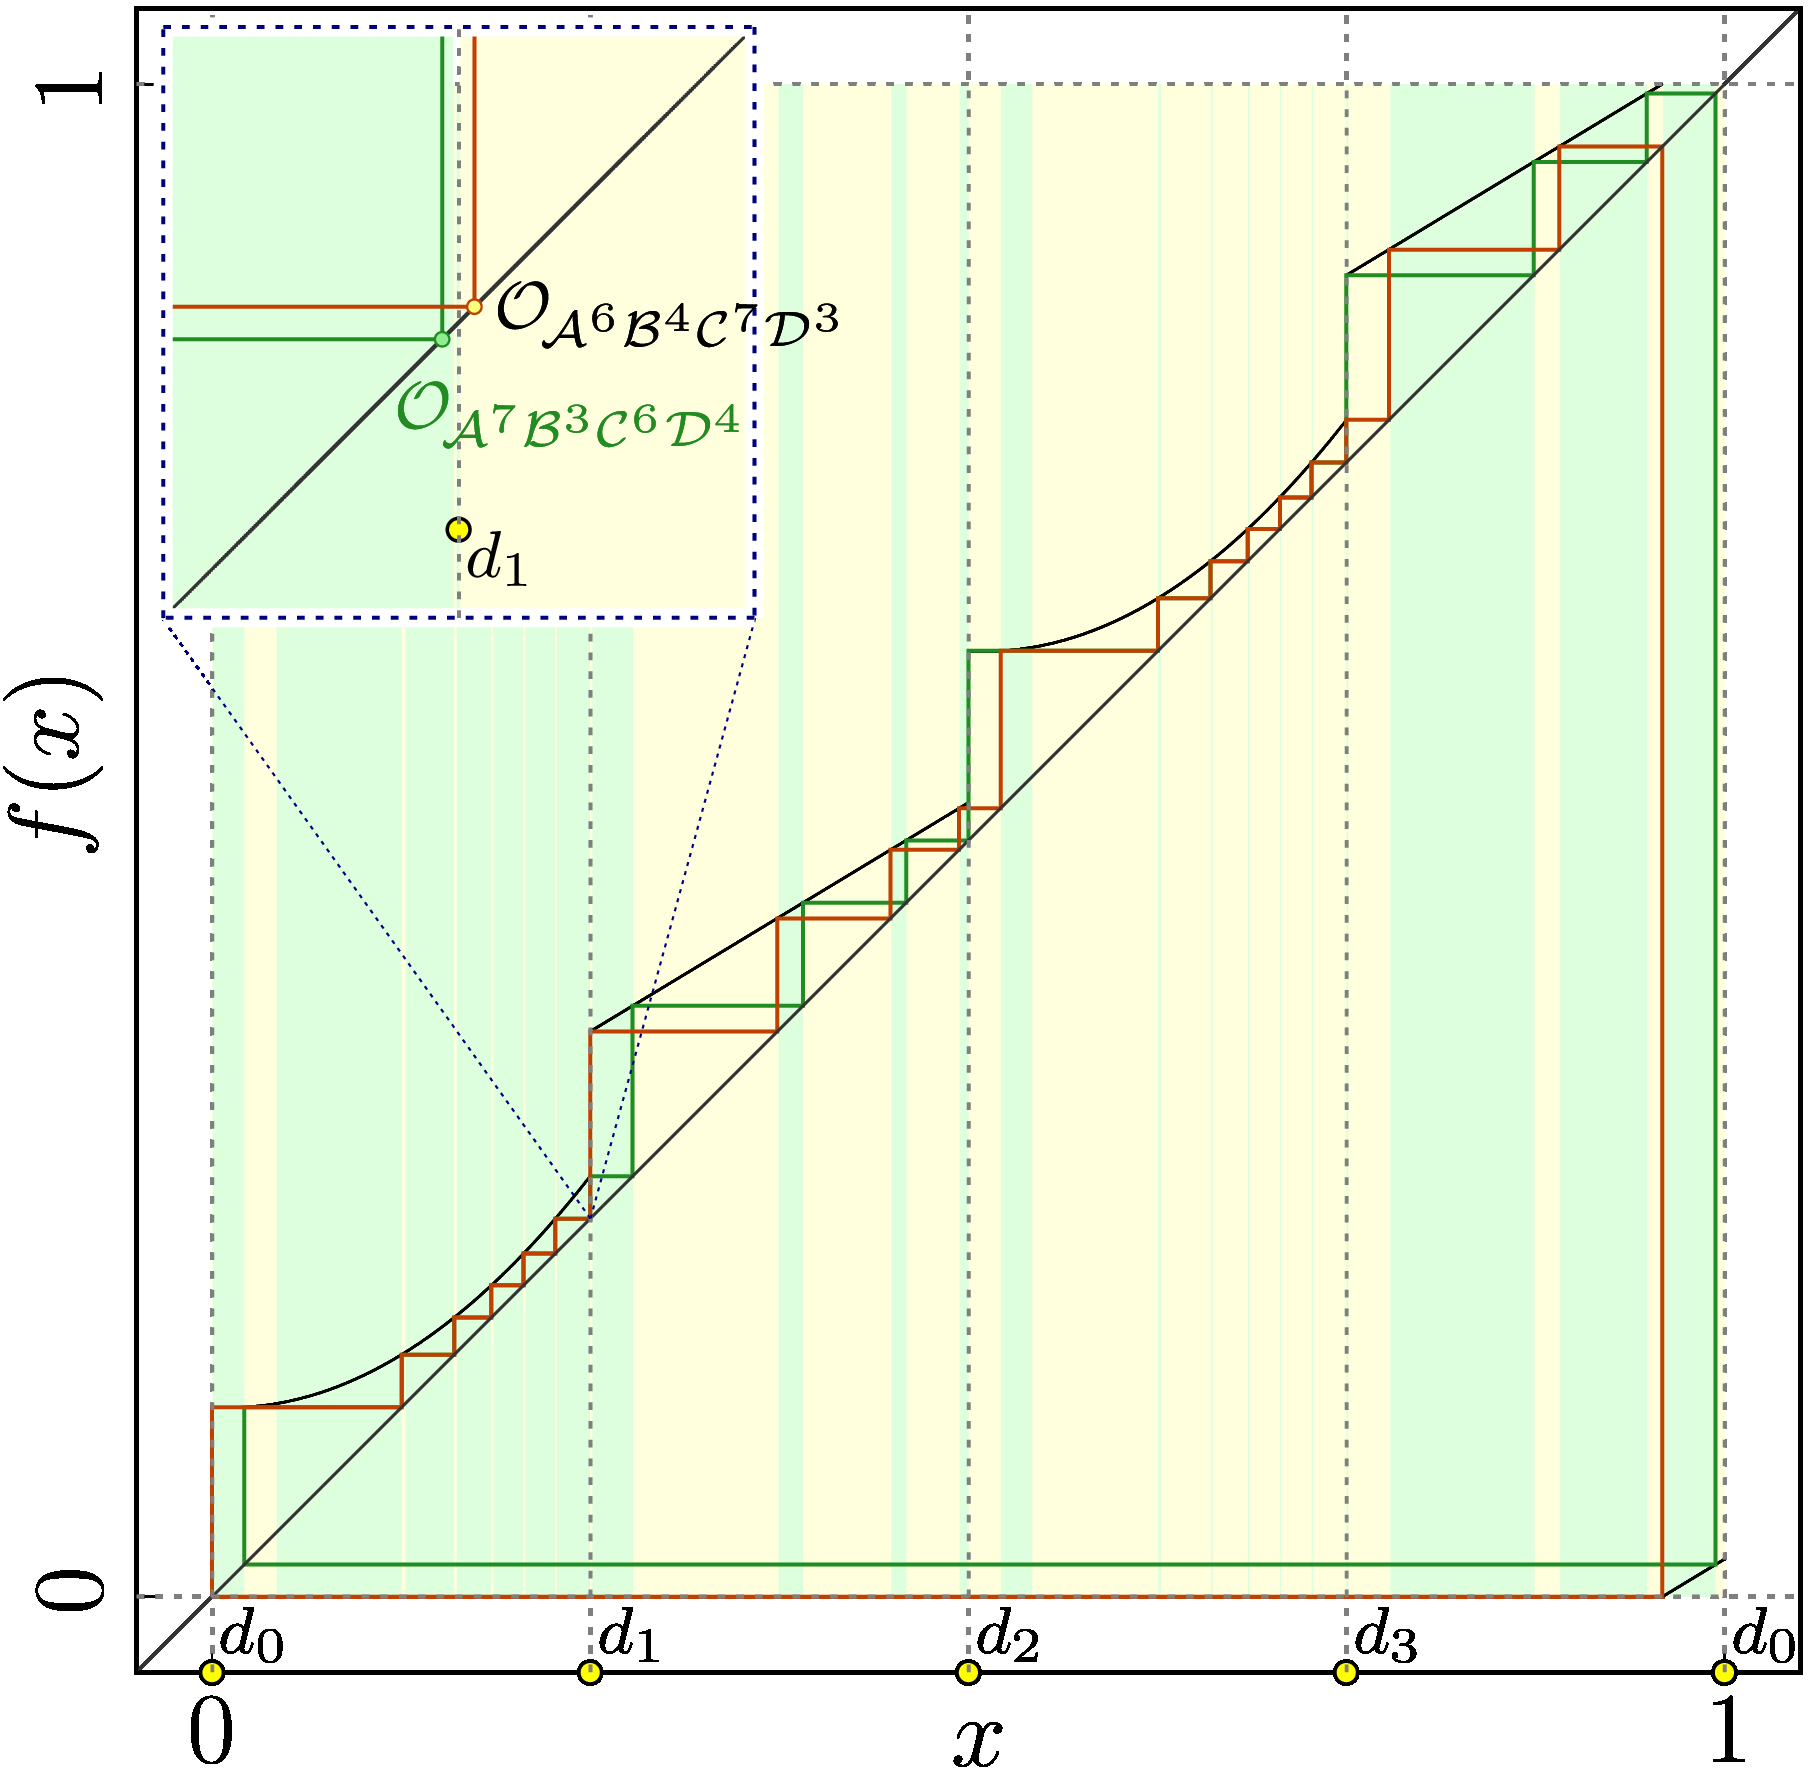
\includegraphics[width=.3 \textwidth]{../Figures/7/7.4c/result.png}
		\label{fig:add.change.disb.cob.B}
	}
	\caption{Disappearance of the ``type B'' parameter region}
\end{figure}

In between those two stages, we can see how the ``type B'' parameter region $Q^{20}_3$ disappears.
\hl{Somewhere along the parameter line given by} \Cref{equ:add.change.paramline} between \Cref{fig:add.change.regions.2} and \Cref{fig:add.change.regions.3}, \hl{the lower left corner of the parameter region $P^{20}_4$ crosses the upper boundary of the parameter region $P^{20}_3$}.
\hl{This causes the ``type A'' parameter regions $P^{20}_3$ and $P^{20}_4$ to overlap in} \Cref{fig:add.change.regions.3}.
\hl{
	The point, where both boundaries cross is not a codimension-2 point, since the bifurcation at the lower boundary of the overlapping parameter region
}
\hl{We know from} \Cref{sec:arch.bif.sum} \hl{that the border collision bifurcation at the upper boundary of $P^{20}_3$ is $\BCB_{d_1, d_3}^{\A^6\underline{\B}^4\C^6\underline{\D}^4}$ and the border collision bifurcation at the lower boundary of $P^{20}_4$ is $\BCB_{d_1, d_3}^{\underline{\A}^7\B^3\underline{\C}^7\D^3}$}.
\hl{
	Therefore, this point is \textbf{not} a codimension-2 point, since the bifurcations happen to different cycle.
	Nonetheless, this is the right corner of the overlapping parameter region of $P^{20}_3 \cap P^{20}_4$.
}

\hl{
	At similar parameter values, where the lower left corner of $P^{20}_4$ crosses the upper boundary of $P^{20}_3$, the upper left corner and the lower left corner of the ``type B'' parameter region $Q^{20}_3$ collide causing the lower and upper boundaries of this parameter region to cross also.
}
\hl{We know from} \Cref{sec:arch.bif.sum} \hl{that the border collision bifurcations at the upper boundary of $Q^{20}_3$ are $\BCB_{d_1}^{\underline{\A}^7\B^3\C^6\D^4}$ and $\BCB_{d_3}^{\A^6\B^4\underline{\C}^7\D^3}$ and the border collision bifurcations at the lower boundary of $Q^{20}_3$ are $\BCB_{d_3}^{\A^7\B^3\C^6\underline{\D}^4}$ and $\BCB_{d_1}^{\A^6\underline{\B}^4\C^7\D^3}$}.
\hl{
	This is a codimension-2 point, since each of the coexisting cycles undergoes two different bifurcations at this point.
}
\hl{Also, this codimension-2 point is different from the codimension-2 points listed in} \Cref{sec:arch.bif.sum}, \hl{since those points always involve all four borders}.
\hl{
	Here, only the borders associated with vertical boundaries, namely $d_1$ and $d_3$, are involved in all four bifurcations at this point.
}

\hl{Along the parameter line given by} \Cref{equ:add.change.paramline} \hl{for increasing values of $b_L$, the lower boundary of $P^{20}_4$ and the upper boundary of $Q^{20}_3$ move down while the upper boundary of $P^{20}_3$ and the lower boundary of $Q^{20}_3$ moves up}.
\hl{
	This leads to both the right corner of the overlapping region $P^{20}_3 \cap P^{20}_4$ and the codimension-2 point which is the left corner of the ``type B'' parameter region $Q^{20}_3$ to move right.
}
\hl{We can observe this movement in} \Cref{fig:add.change.disb.regions}.
\hl{
	Here, those two corner points are near the right boundaries of $Q^{20}_3$ and $P^{20}_3$.
	As soon as the codimension-2 point of the boundaries ``type B'' parameter region crosses the right boundary of the ``type B'' parameter region, the ``type B'' parameter region vanishes.
	And as soon as the right corner point of the overlapping parameter region $P^{20}_3 \cap P^{20}_4$ collides with the upper right corner of $P^{20}_3$, the upper boundary of $P^{20}_3$ stops crossing the lower boundary $P^{20}_4$ and the overlapping parameter region $P^{20}_3 \cap P^{20}_4$ has four boundaries instead of three.
}
